\documentclass[12pt]{extarticle}
%Some packages I commonly use.
\usepackage[english]{babel}
\usepackage{graphicx}
\usepackage{framed}
\usepackage[normalem]{ulem}
\usepackage{amsmath}
\usepackage{amsthm}
\usepackage{amssymb}
\usepackage{amsfonts}
\usepackage{enumerate}
\usepackage[utf8]{inputenc}
\usepackage{listings}
\usepackage[top=1 in,bottom=1in, left=1 in, right=1 in]{geometry}
\usepackage{color}
\usepackage{float}

\definecolor{dkgreen}{rgb}{0,0.6,0}
\definecolor{gray}{rgb}{0.5,0.5,0.5}
\definecolor{mauve}{rgb}{0.58,0,0.82}

%A bunch of definitions that make my life easier
\newcommand{\matlab}{{\sc Matlab} }
\newcommand{\cvec}[1]{{\mathbf #1}}
\newcommand{\rvec}[1]{\vec{\mathbf #1}}
\newcommand{\ihat}{\hat{\textbf{\i}}}
\newcommand{\jhat}{\hat{\textbf{\j}}}
\newcommand{\khat}{\hat{\textbf{k}}}
\newcommand{\minor}{{\rm minor}}
\newcommand{\trace}{{\rm trace}}
\newcommand{\spn}{{\rm Span}}
\newcommand{\rem}{{\rm rem}}
\newcommand{\ran}{{\rm range}}
\newcommand{\range}{{\rm range}}
\newcommand{\mdiv}{{\rm div}}
\newcommand{\proj}{{\rm proj}}
\newcommand{\R}{\mathbb{R}}
\newcommand{\N}{\mathbb{N}}
\newcommand{\Q}{\mathbb{Q}}
\newcommand{\Z}{\mathbb{Z}}
\newcommand{\<}{\langle}
\renewcommand{\>}{\rangle}
\renewcommand{\emptyset}{\varnothing}
\newcommand{\attn}[1]{\textbf{#1}}
\theoremstyle{definition}
\newtheorem{theorem}{Theorem}
\newtheorem{corollary}{Corollary}
\newtheorem*{definition}{Definition}
\newtheorem*{example}{Example}
\newtheorem*{note}{Note}
\newtheorem{exercise}{Exercise}
\newcommand{\bproof}{\bigskip {\bf Proof. }}
\newcommand{\eproof}{\hfill\qedsymbol}
\newcommand{\Disp}{\displaystyle}
\newcommand{\qe}{\hfill\(\bigtriangledown\)}
\setlength{\columnseprule}{1 pt}

\lstset{frame=tb,
	language=C,
	aboveskip=3mm,
	belowskip=3mm,
	showstringspaces=false,
	columns=flexible,
	basicstyle={\small\ttfamily},
	numbers=none,
	numberstyle=\tiny\color{gray},
	keywordstyle=\color{blue},
	commentstyle=\color{dkgreen},
	stringstyle=\color{mauve},
	breaklines=true,
	breakatwhitespace=true,
	tabsize=3
}

\title{CS307 Project2: Unix Shell Programming \& LKM for task information}
\author{Junjie Wang 517021910093}

\begin{document}
	\maketitle 
	\section{Programming Thoughts}
	\subsection{Part 1: Unix Shell Programming}
	The main logic is to use a while loop to get inputs from the user. Then create a child process(using $fork()$) to execute the command. \\
	To support the history logic, we simply need to maintain one more variable($char *last\_input)$. And when receving $'!!'$, copy $last\_input$ into the $input$ string.\\ 
	To support the \& logic, we simply need to modify a little bit about the behavior of the parent process(do not wait until the child process exits). Another thing worth attention here is using $signal()$ to prevent the \textbf{zombies}.\\
	To support the redirection logic, the idea is to use $dup2()$ function, closing the stdin/stdout file descriptors and reset its pointer according to the file descriptor we are going to open(e.g. output.txt). \\
	To support the pipe($'|'$), the idea is to create the child process of the child process(also using $fork()$). Pipe is acommplished through the IPC between these two processes. $dup()$ function is used here, actually quite similar to the $dup2()$.
	\subsection{Part 2: Linux Kernel Module For Task Information}
	The idea is to get the pid from user's input in $proc\_write()$ function. Then use $task\_pid()$ to get corresponding process and output the pid, command and state of this process. Another thing worth attention is that there should be a logic to handle invalid pid(simply return 0);
	\section{Execution Results And Snapshots}
	Execution results are shown as belows:
	\begin{figure}[H]
		\centering 
		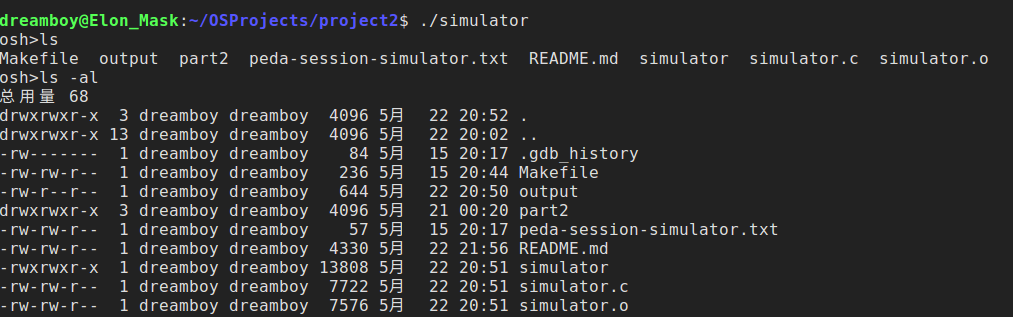
\includegraphics[width=0.8\textwidth]{../imgs/2-1.png}
		\label{fig1}
		\caption{Primitive Version}
	\end{figure}
	\begin{figure}[H]
		\centering 
		\includegraphics[width=0.8\textwidth]{../imgs/2-4.png}
		\label{fig2}
		\caption{Add support for history feature}
	\end{figure}
	\begin{figure}[H]
		\centering 
		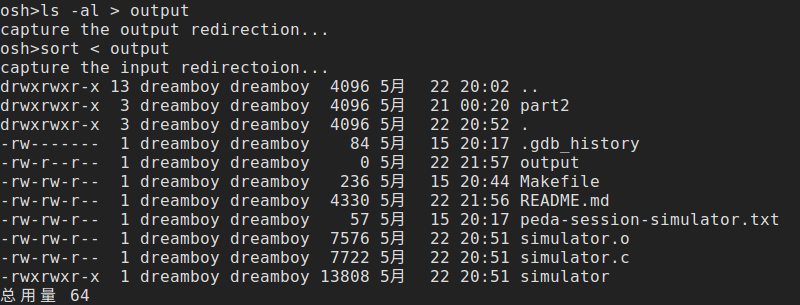
\includegraphics[width=0.8\textwidth]{../imgs/2-2.png}
		\label{fig3}
		\caption{Add support for \& and the redirection}
	\end{figure}
	\begin{figure}[H]
		\centering 
		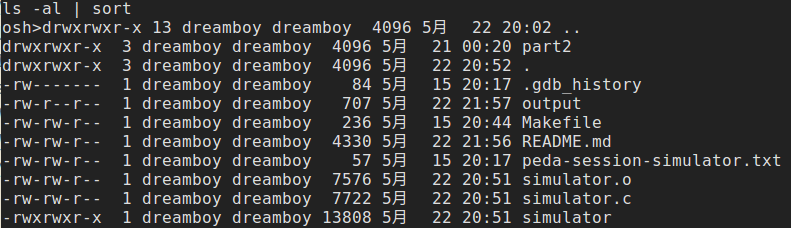
\includegraphics[width=0.8\textwidth]{../imgs/2-3.png}
		\label{fig4}
		\caption{Add support for the pipe}
	\end{figure}
	\begin{figure}[H]
		\centering 
		\includegraphics[width=0.8\textwidth]{../imgs/2-5.png}
		\label{fig5}
		\caption{The part 2, LKM for task information}
	\end{figure}
	\section{Code Explanation}
	\subsection{part 1}
		An important part is using the $dup()$, $dup2()$ and $execvp()$ functions.
		\begin{lstlisting}
		/* find a minimum value in current available file descriptors and set its pointer as the oldfd */
		int dup(int oldfd);
		/* only a little different from dup(). In dup2() we can specify the newfd we want to use. It newfd is already open, close it first */
		int dup2(int oldfd, int newfd);
		/* exec family functions. Note that the first file parameter will be search in $(PATH) environment variable and the last parameter for the */
		int execvp(const char *file, const char *argv[]);
		\end{lstlisting}
		The logic for the pipe is as follows. For the child process, we first close the stdin and the write port of the pipe. Then use $dup()$ function to get the $0$ file descriptor and set its pointer to the read port of the pipe. The logic for the parent process is similar.
		\begin{lstlisting}
		int p[2], ppid;
		
		pipe(p);
		ppid = fork();
		if(ppid < 0)    {perror("ppid create error!");exit(1);}
		else if(ppid == 0){
		/* for the child of the child process, set it as the executor of the second commmand */
		close(0);
		close(p[1]);
		if(dup(p[0]) < 0)   {perror("dup error!");exit(1);}
		res = execvp(pipe_args[0], pipe_args);
		if(res < 0) { perror("cmd2 execution error!"); exit(1); }
		}else{
		/* for the parent process, it will execute the first command */
		/* close stdout */
		close(1);
		/* close one port */
		close(p[0]);
		if(dup(p[1]) < 0)   {perror("dup error!");exit(1);}
		res = execvp(valid_args[0], valid_args);
		if(res < 0) { perror("cmd1 execution error!"); exit(1); }
		}
		\end{lstlisting}
	\subsection{part 2}
		To get the $command, state, pid$ information, we need to refer to $linux/sched.h$ and use logic as follows in $proc\_read()$ function(Note that $l\_pid$ is parsed from $proc\_write()$ function.
		\begin{lstlisting}
		static ssize_t proc_read(struct file *file, char __user *usr_buf, size_t count, loff_t *pos)
		{
		int rv = 0;
		char buffer[BUFFER_SIZE];
		static int completed = 0;
		struct task_struct *tsk = NULL;
		
		if (completed) {
		completed = 0;
		return 0;
		}
		
		tsk = pid_task(find_vpid(l_pid), PIDTYPE_PID);
		
		completed = 1;
		
		/* return 0 if no this pid */
		if( tsk == NULL)    return 0;
		else rv = sprintf(buffer, "command = %s pid = %d state = %ld\n", tsk->comm, tsk->pid, tsk->state);
		
		// copies the contents of kernel buffer to userspace usr_buf 
		if (copy_to_user(usr_buf, buffer, rv)) {
		rv = -1;
		}
		
		return rv;
		}
		\end{lstlisting}
	
\end{document}